\section{概述}
\begin{enumerate}
	\item 目的:系统掌握数字系统的基本概念、思维模式与设计方法,帮助深入理解计算机架构
	\item 应用:
	\begin{itemize}
		\item 人工智能+GPU/FPGA
		\item 云计算+FPGA
		\item 物联网+传感硬件系统
		\item 软件定义网络系统
	\end{itemize}
\end{enumerate}


\section{基本概念}
\subsection{数字与模拟}
\begin{enumerate}
	\item 数字(digital)量:离散值,01
	\item 模拟(analog)量:连续值
\end{enumerate}

\subsection{数的表示}
\subsubsection{进制(system)}
二进制(binary)、八进制(octonary)、十进制(decimal)、十六进制(hexadecimal)
\begin{itemize}
	\item 十进制转二进制:整数部分除以2取余,小数部分乘2取整
	\item 二进制转十六进制:四位四位统计
\end{itemize}
\subsubsection{符号数}
\begin{itemize}
	\item 符号数值(sign-magnitude)形式:首位0为正数,1为负数,n位范围为$-(2^{n-1}-1)\thicksim +2^{n-1}-1$
	\item 反码(1's complement):除符号位不变,其他位取反,n位范围为$-(2^{n-1}-1)\thicksim +2^{n-1}-1$
	\item 补码(2's complement):反码+1,按照原来十进制转二进制方法即可得对应有符号十进制数,n位范围为$\color{red}{-2^{n-1}}$$\thicksim +2^{n-1}-1$(由于没有正负0,故表示的数多了一位),补码的补码为原码
\end{itemize}
\subsubsection{浮点数}
单精度(float)32位,双精度(double)64位
\par 指数加127相当于做了一个平移,科学记数法如下表示,
\[\text{Number}=(-1)^S(1+F)2^{E-127}\]
\begin{example}
\[1\;0110\;1001\;0001=1.0110\;1001\;0001\times 2^{12}\]
\par 指数:$12+127=139\to 1000\;1011$
\par 尾数:$011\;0100\;1000\;1000\;0000\;0000$ 左对齐,因为有小数点
\begin{center}
\begin{tabular}[htbp]{|c|c|c|}
\hline
符号S & 指数E(exponent) & 尾数F(mantissa)\\\hline
$0$ & $1000\;1011$ & $011\;0100\;1000\;1000\;0000\;0000$\\\hline
1位 & 8位 & 23位\\\hline
\end{tabular}
\end{center}
\end{example}
\subsubsection{运算法则}
用补码进行计算,操作跟原码相同,且不会出现两个0
\subsubsection{其他表示}
\begin{enumerate}
	\item BCD码/8421码:即四位的二进制表示
	\item 格雷(Gray)码:相邻只变一位
\end{enumerate}
\par 二进制码转格雷码:
\begin{center}
\begin{tikzcd}
Binary: & 1\arrow{d}\arrow{r}{+} & 0\arrow{d}\arrow{r}{+} & 1\arrow{d}\arrow{r}{+} & 1\arrow{d}\arrow{r}{+} & 0\arrow{d}\\
Gray: & 1 & 1 & 1 & 0 & 1
\end{tikzcd}
\end{center}
\par 格雷码转二进制码:
\begin{center}
\begin{tikzcd}
Gray: & 1\arrow{d} & 1\arrow{d} & 1\arrow{d} & 0\arrow{d} & 1\arrow{d}\\
Binary: & 1\arrow{ur}{+} & 0\arrow{ur}{+} & 1\arrow{ur}{+} & 1\arrow{ur}{+} & 0
\end{tikzcd}
\end{center}

\subsection{存储器}
\subsubsection{随机存取存储器(RAM)}
\begin{itemize}
	\item 静态(SRAM):用锁存器作为存储单元,只要有电源就可以一直存,读快
	\item 动态(DRAM):用电容器作为存储单元,需要不断刷新(refreshing),存储容量大
\end{itemize}
\subsubsection{只读存储器(ROM)}
永久或半永久存储数据
\subsubsection{存储扩展}
\begin{itemize}
	\item 字长(word-length)扩展
\begin{figure}[htbp]
	\centering
	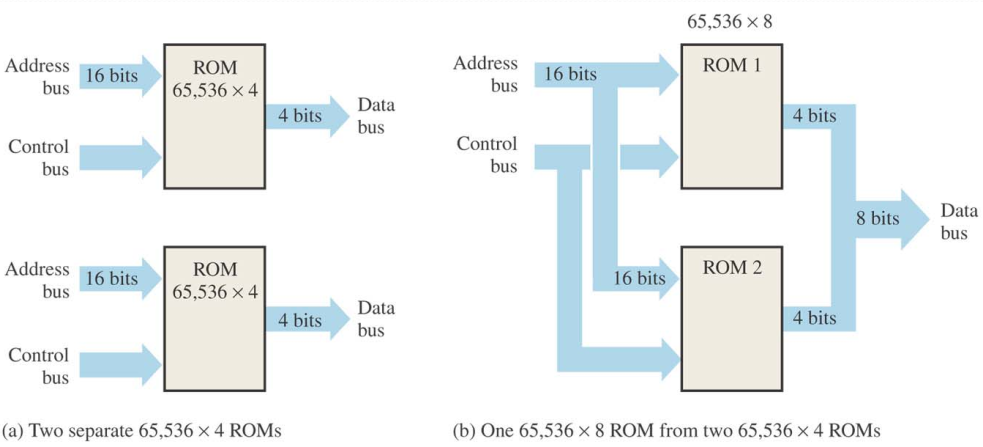
\includegraphics[width=0.6\linewidth]{fig/word-length.PNG}
	\caption{字长扩展}
\end{figure}
	\item 字容量(word-capacity)扩展
\begin{figure}[htbp]
	\centering
	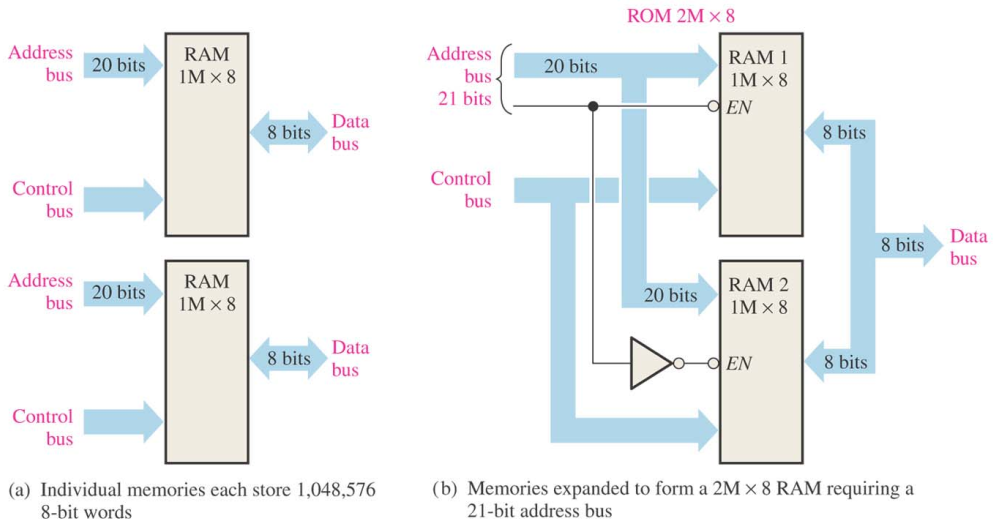
\includegraphics[width=0.6\linewidth]{fig/word-capacity.PNG}
	\caption{字容量扩展}
\end{figure}
\end{itemize}

\subsection{信号处理}
\begin{enumerate}
	\item 采样(sampling)\\
	采样频率至少是原来最高频率的两倍
	\item 滤波(filtering)\\
	奈奎斯特(Nyquist)频率等于采样频率的一半
\end{enumerate}

\subsection{其他}
\begin{figure}[htbp]
\begin{minipage}{0.5\linewidth}
	\centerline{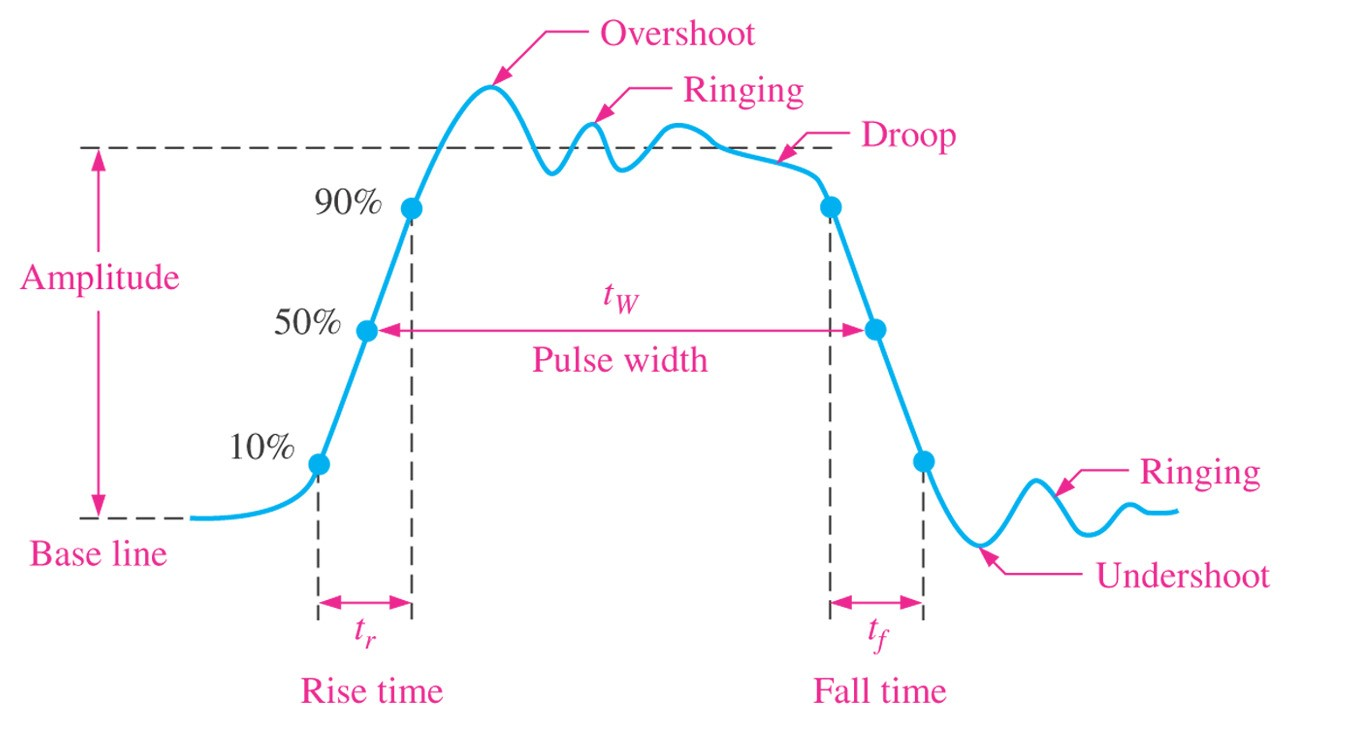
\includegraphics[width=\linewidth]{fig/nonideal_pulse_characteristics.jpg}}
	\centerline{非理想脉冲}
\end{minipage}
\begin{minipage}{0.5\linewidth}
	\centerline{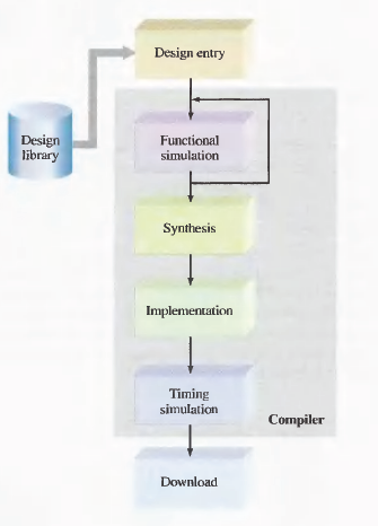
\includegraphics[width=0.6\linewidth]{fig/design_flow.png}}
	\centerline{设计流}
\end{minipage}
\end{figure}
占空比(duty cycle):$\dfrac{t_W}{T}\times 100\%$